% gm-09-TrigEqs.tex

\documentclass[xcolor=dvipsnames]{beamer}

\usepackage{cancel}
\renewcommand{\CancelColor}{\color{red}}
\usepackage{graphicx}
\usepackage{wrapfig}
\usepackage{colortbl}
\usepackage{color}
\usepackage{alltt}
\renewcommand*{\thefootnote}{\fnsymbol{footnote}}
\definecolor{myblue}{rgb}{0.8,0.85,1}

\mode<presentation>
{
  \usetheme{Warsaw}
  \setbeamercovered{transparent}
}
% \usecolortheme[named=OliveGreen]{structure}
\setbeamertemplate{navigation symbols}{} 
\setbeamertemplate{blocks}[rounded][shadow=true] 

% this is for overlaying math symbols, see https://tex.stackexchange.com/questions/12895/overlay-symbol-with-another
\def\qeq{\mathrel{%
    \mathchoice{\QEQ}{\QEQ}{\scriptsize\QEQ}{\tiny\QEQ}%
}}
\def\QEQ{{%
    \setbox0\hbox{$\longrightarrow$}%
    \rlap{\hbox to \wd0{\hss/\hss}}\box0
  }}

\newcounter{expls}
\setcounter{expls}{0}
\newcommand{\beispiel}[1]{\refstepcounter{expls}\textbf{Example \arabic{expls}: #1.}}

\newcounter{exercise}
\setcounter{exercise}{0}
\newcommand{\ubung}[0]{\refstepcounter{exercise}\textbf{Exercise \arabic{exercise}: }}

\newif\ifBCITCourse
\BCITCoursetrue
% \BCITCoursefalse
\newif\ifWhichCourse
\WhichCoursetrue
\WhichCoursefalse
\ifBCITCourse
\ifWhichCourse
\newcommand{\CourseName}{Technical Mathematics for Food Technology}
\newcommand{\CourseNumber}{MATH 1441}
\newcommand{\CourseInst}{BCIT}
\else
\newcommand{\CourseName}{Technical Mathematics for Geomatics}
\newcommand{\CourseNumber}{MATH 1511}
\newcommand{\CourseInst}{BCIT}
\fi
\else
\newcommand{\CourseName}{Philosophy and Literature}
\newcommand{\CourseNumber}{PHIL 375}
\newcommand{\CourseInst}{UBC}
\fi

\title{Trigonometric Equations}
\subtitle{{\CourseNumber}, BCIT}

\author{\CourseName}

\date{October 17, 2017}

\begin{document}

\begin{frame}
  \titlepage
\end{frame}

\begin{frame}
  \frametitle{Trigonometric Equations}
\beispiel{Trigonometric Equation with Sine and Cosine} Solve the following trigonometric equation,
\begin{equation}
  \label{eq:yeobidae}
  1+\sin\vartheta=2\cos^{2}\vartheta
\end{equation}  
It is often a good strategy to convert everything to either sine or
cosine and then solve for the unknown $\sin\vartheta$ or
$\cos\vartheta$. In this case, for example, write
\begin{equation}
  \label{eq:aegovatu}
  1+\sin\vartheta=2(1-\sin^{2}\vartheta)
\end{equation}
and then replace $\sin\vartheta=x$ (this method is sometimes called
substitution). Therefore,
\begin{equation}
  \label{eq:aequeete}
2x^{2}+x-1=0  
\end{equation}
\end{frame}

\begin{frame}
  \frametitle{Trigonometric Equations}
  The solutions for equation (\ref{eq:aequeete}) are
  \begin{equation}
    \label{eq:koshoepi}
    x=-1\mbox{ or }x=\frac{1}{2}
  \end{equation}
  Now revert to the meaning of $x=\sin\vartheta$. Therefore,
  \begin{equation}
    \label{eq:hutahkig}
    \sin\vartheta=-1\mbox{ or }\sin\vartheta=\frac{1}{2}
  \end{equation}
Then take the multiple solutions into account that exist within one period
of the sine, for example $[0,2\pi)$.
\begin{equation}
  \label{eq:ciowoowu}
  \vartheta=30^{\circ}\mbox{ or }\vartheta=150^{\circ}\mbox{ or }\vartheta=270^{\circ}
\end{equation}
\end{frame}

\begin{frame}
  \frametitle{Trigonometric Equations}
Consider the period of the trigonometric function (sine, in
this case) to finalize the solution set.
\begin{equation}
  \label{eq:phahchoh}
  S=\{\vartheta\in\mathbb{R}|\vartheta=30^{\circ}+k\cdot{}360^{\circ},\vartheta=150^{\circ}+k\cdot{}360^{\circ},\notag
\end{equation}
\begin{equation}
  \label{eq:rerushao}
  \vartheta=270^{\circ}+k\cdot{}360^{\circ},k\in\mathbb{Z}\}
\end{equation}
It is easy to miss solutions, so it is a good idea to check that you
have them all in a function graph. Here is my input on
\texttt{www.desmos.com}
  \begin{figure}[h]
    \includegraphics[scale=.4]{./trigeqdesmos2.png}
  \end{figure}
  Look at the function graph on the next slide and compare the
  intersections to the solution set.
\end{frame}

\begin{frame}
  \frametitle{Trigonometric Equations}
  \begin{figure}[h]
    \includegraphics[scale=.4]{./trigeqdesmos1.png}
  \end{figure}
\end{frame}

\begin{frame}
  \frametitle{Trigonometric Equations}
\beispiel{Trigonometric Equation with Tangent and Cotangent} Solve the following trigonometric equation,
\begin{equation}
  \label{eq:leegaexu}
\tan{}2\vartheta=\cot\vartheta
\end{equation}
It may be helpful to turn these trigonometric functions immediately
into sines and cosines.
\begin{equation}
  \label{eq:jautithe}
  \frac{\sin{}2\vartheta}{\cos{}2\vartheta}=\frac{cos\vartheta}{\sin\vartheta}
\end{equation}
Now use the double-angle formula
\begin{equation}
  \label{eq:yaamieya}
  \frac{2\sin\vartheta\cos\vartheta}{\cos^{2}\vartheta-\sin^{2}\vartheta}=\frac{cos\vartheta}{\sin\vartheta}
\end{equation}
\end{frame}

\begin{frame}
  \frametitle{Trigonometric Equations}
  Use cross-multiplication for
  \begin{equation}
    \label{eq:eegheico}
    2\sin^{2}\vartheta\cos\vartheta=(\cos^{2}\vartheta-\sin^{2}\vartheta)\cos\vartheta
  \end{equation}
Shift everything to the left-hand side and factor out $\cos\vartheta$
for
\begin{equation}
  \label{eq:paeghohf}
  \cos\vartheta\cdot(3\sin^{2}\vartheta\cos\vartheta-cos^{2}\vartheta)=0
\end{equation}
There are two factors here that multiply to give us zero. Look at
them individually when they might turn zero.
\begin{equation}
  \label{eq:ielaepoo}
  \cos\vartheta=0\mbox{ or }3\sin^{2}\vartheta-\cos^{2}\vartheta=0
\end{equation}
Replace $\cos^{2}\vartheta$ by $1-\sin^{2}\vartheta$ in the second
factor for $\sin\vartheta=1/2$ or $\sin\vartheta=1/2=-1/2$.
\end{frame}

\begin{frame}
  \frametitle{Trigonometric Equations}
Consequently,
\begin{equation}
  \label{eq:athaelae}
  \vartheta=90^{\circ}\mbox{ or }\vartheta=270^{\circ}\mbox{ or }\notag
\end{equation}
\begin{equation}
  \label{eq:eehohbei}
  \vartheta=30^{\circ}\mbox{ or }\vartheta=150^{\circ}\mbox{ or }\notag
\end{equation}
\begin{equation}
  \label{eq:yaelivei}
  \vartheta=210^{\circ}\mbox{ or }\vartheta=330^{\circ}
\end{equation}
Therefore, the solution set is
\begin{equation}
  \label{eq:vohhaewe}
  S=\{\vartheta\in\mathbb{R}|\vartheta=30^{\circ}+k\cdot{}180^{\circ},\vartheta=90^{\circ}+k\cdot{}180^{\circ},\notag
\end{equation}
\begin{equation}
  \label{eq:aleichou}
  \vartheta=150^{\circ}+k\cdot{}180^{\circ},k\in\mathbb{Z}\}
\end{equation}
Notice that the period is now $180^{\circ}$, which is what we would
expect from a trigonometric equation with tangents and cotangents.
\end{frame}

\begin{frame}
  \frametitle{Trigonometric Equations}
    \begin{figure}[h]
    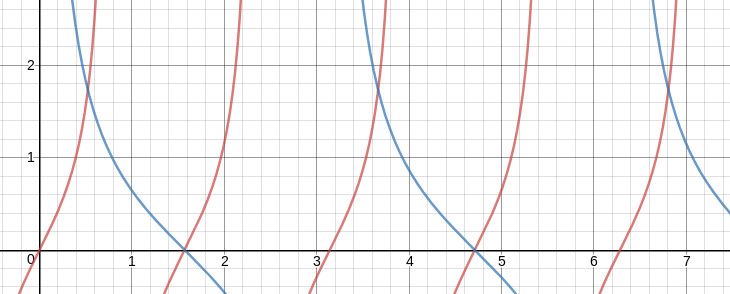
\includegraphics[scale=.4]{./trigeqdesmos3.png}
  \end{figure}
\end{frame}

\begin{frame}
  \frametitle{Trigonometric Equations}
\beispiel{Trigonometric Equation with Modified Angles} Solve the following trigonometric equation,
\begin{equation}
  \label{eq:nihezoof}
  2\sin{}3\vartheta-1=0
\end{equation}  
We could use a formula for the triple angle here,
\begin{equation}
  \label{eq:aophatou}
  \sin{}3\vartheta=\sin(2\vartheta+\vartheta)=\sin{}2\vartheta\cos\vartheta+\sin\vartheta\cos{}2\vartheta=\notag
\end{equation}
\begin{equation}
  \label{eq:eilohbei}
  2\sin\vartheta\cos\vartheta\cdot\cos\vartheta+\sin\vartheta(\cos^{2}\vartheta-\sin^{2}\vartheta)
\end{equation}
but this expression looks daunting.
\end{frame}

\begin{frame}
  \frametitle{Trigonometric Equations}
  Instead, substitute $\alpha=3\vartheta$ for
  \begin{equation}
    \label{eq:aefufahw}
  2\sin\alpha-1=0
  \end{equation}
  The solutions are
  \begin{equation}
    \label{eq:noocheiy}
    \alpha={\ldots},30^{\circ},150^{\circ},390^{\circ},510^{\circ},{\ldots}
  \end{equation}
  Therefore,
  \begin{equation}
    \label{eq:beiseith}
\vartheta={\ldots},10^{\circ},50^{\circ},130^{\circ},170^{\circ},{\ldots}
  \end{equation}
Notice how the period has changed from $360^{\circ}$ to $120^{\circ}$.
\begin{equation}
  \label{eq:aereukiu}
  S=\{\vartheta\in\mathbb{R}|\vartheta=10^{\circ}+k\cdot{}120^{\circ},\vartheta=50^{\circ}+k\cdot{}120^{\circ},k\in\mathbb{Z}\}
\end{equation}
\end{frame}

\begin{frame}
  \frametitle{Trigonometric Equations}
    \begin{figure}[h]
    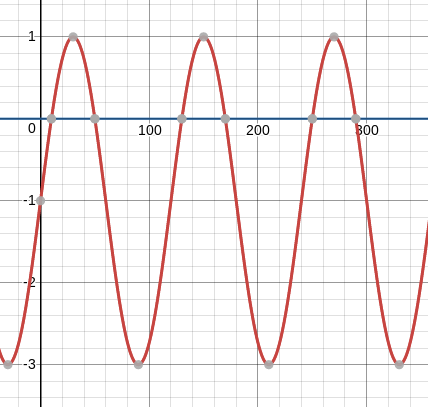
\includegraphics[scale=.55]{./trigeqdesmos4.png}
  \end{figure}
\end{frame}

\begin{frame}
  \frametitle{Trigonometric Equations}
{\ubung} Solve the following trigonometric equation,
\begin{equation}
  \label{eq:iefojaes}
  2\sin\vartheta-1=0
\end{equation}
\end{frame}

\begin{frame}
  \frametitle{Trigonometric Equations}
{\ubung} Solve the following trigonometric equation,
\begin{equation}
  \label{eq:ahgaofoo}
  (\cot^{2}\vartheta)(3+\sqrt{5})+\sqrt{5}=5
\end{equation}  
\end{frame}

\begin{frame}
  \frametitle{Trigonometric Equations}
{\ubung} Solve the following trigonometric equation,
\begin{equation}
  \label{eq:aeciengo}
  2\cos^{2}\vartheta-7\cos\vartheta+3=0
\end{equation}  
\end{frame}

\begin{frame}
  \frametitle{Trigonometric Equations}
{\ubung} Solve the following trigonometric equation,
  \begin{equation}
  \label{eq:taicaite}
  \cos{}2\vartheta=\sqrt{3}-\sin\vartheta
\end{equation}
\end{frame}

\begin{frame}
  \frametitle{Trigonometric Equations}
{\ubung} Solve the following trigonometric equation,
\begin{equation}
  \label{eq:ohyeikei}
  \sqrt{3}\tan\frac{\vartheta}{2}-1=0
\end{equation}  
\end{frame}

\begin{frame}
  \frametitle{Trigonometric Equations}
{\ubung} Solve the following trigonometric equation,
\begin{equation}
  \label{eq:ahwasohw}
  \tan^{2}\vartheta-\tan\vartheta-2=0
\end{equation}  
\end{frame}

\begin{frame}
  \frametitle{Trigonometric Equations}
  {\ubung} Solve the following trigonometric equation,
\begin{equation}
  \label{eq:ohtheinu}
  \sin{}3\vartheta+\sin\vartheta=0
\end{equation}
\end{frame}

\begin{frame}
  \frametitle{Trigonometric Equations}
  {\ubung} Solve the following trigonometric equation,
\begin{equation}
  \label{eq:ioshaoqu}
2\sin^{2}\frac{1}{2}\vartheta-\cos\vartheta=2
\end{equation}
\end{frame}

\begin{frame}
  \frametitle{Trigonometric Equations}
  {\ubung} Solve the following trigonometric equation,
\begin{equation}
  \label{eq:taepuhee}
\sec{}2\vartheta=2\cos\vartheta-1
\end{equation}
\end{frame}

\begin{frame}
  \frametitle{Trigonometric Equations}
  {\ubung} Solve the following trigonometric equation,
\begin{equation}
  \label{eq:eyeepiiz}
\sin^{2}\vartheta-\cos^{2}\vartheta-\cos{}2\vartheta=1
\end{equation}
\end{frame}

\begin{frame}
  \frametitle{Trigonometric Equations}
  {\ubung} Solve the following trigonometric equation,
\begin{equation}
  \label{eq:deechahk}
2\sin\left(\vartheta-\frac{\pi}{6}\right)=\sqrt{3}\sin\vartheta
\end{equation}
\end{frame}

\begin{frame}
  \frametitle{End of Lesson}
Next Lesson: Conics.
\end{frame}

\end{document}
